\chapter{Emboss}

\section{Performance Tests}

\begin{center}
    \begin{figure}[H]
        \centering
        
        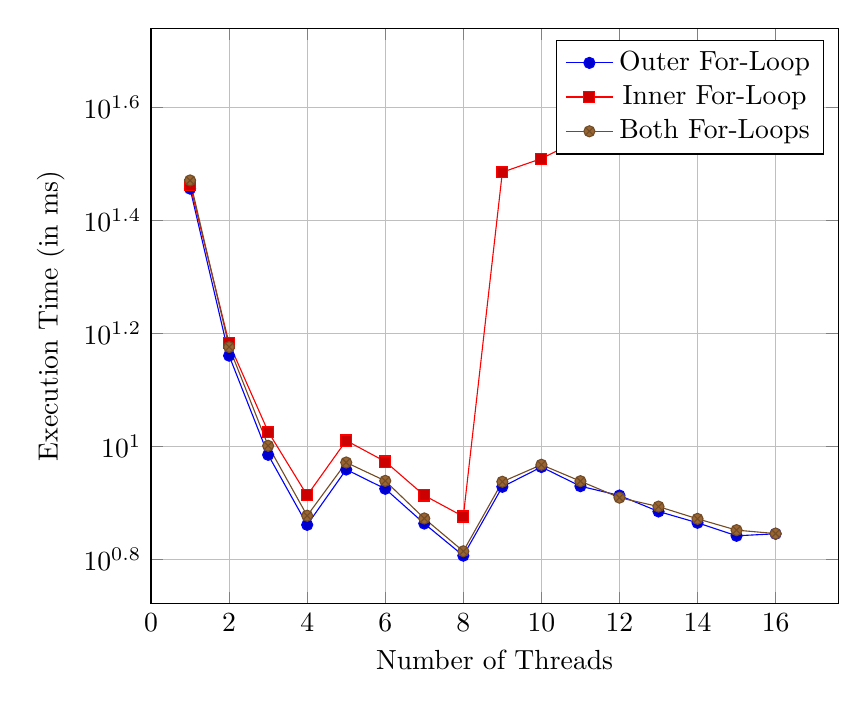
\begin{tikzpicture}
            \begin{axis}[
                title={},
                width=0.85\textwidth,
                xlabel={Number of Threads},
                ylabel={Execution Time (in ms)},
                xmin=0,
                ymin=0,
                ymode=log,
                grid=major
            ]
                \addplot coordinates {
                    (1,28.5583)(2,14.4724)(3,9.66625)(4,7.2702)(5,9.1055)(6,8.4178)(7,7.30745)(8,6.41185)(9,8.48695)(10,9.19905)(11,8.508)(12,8.1918)(13,7.677)(14,7.33135)(15,6.95245)(16,7.0099)
                };
                \addlegendentry{Outer For-Loop}

                \addplot coordinates {
                    (1,28.9709)(2,15.213)(3,10.6239)(4,8.1958)(5,10.2444)(6,9.4047)(7,8.1935)(8,7.52165)(9,30.54)(10,32.2743)(11,34.9379)(12,35.3693)(13,37.9348)(14,39.7072)(15,41.118)(16,45.1394)
                };
                \addlegendentry{Inner For-Loop}

                \addplot coordinates {
                    (1,29.5323)(2,14.9916)(3,10.0283)(4,7.545)(5,9.3703)(6,8.69475)(7,7.4621)(8,6.5289)(9,8.66325)(10,9.2846)(11,8.6837)(12,8.11935)(13,7.8319)(14,7.4501)(15,7.115)(16,7.01605)
                };
                \addlegendentry{Both For-Loops}
            \end{axis}
        \end{tikzpicture}
    \caption{Emboss Performance Tests}
    \end{figure}
\end{center}

\section{Results}

\begin{figure}[H]
    \centering

    \includegraphics[width=0.25\textwidth]{images/dice.png}
    \includegraphics[width=0.25\textwidth]{images/own-emboss.png}
    
    \caption{Results of self-implemented Emboss-Algorithm}
    \label{fig:emboss}
\end{figure}

\section{Implementation}

\begin{listing}[H]
    \begin{minted}{cpp}
cv::Mat applyEmbossOuter(cv::Mat srcImage, int numThreads = omp_get_num_procs()) {
    cv::Mat destImage(srcImage.rows, srcImage.cols, CV_8UC1);
    omp_set_num_threads(numThreads);

    #pragma omp parallel for default(none) shared(srcImage, destImage)
    for (int row = 0; row < srcImage.rows; row++) {
        for (int col = 0; col < srcImage.cols; col++) {
            int diffR, diffG, diffB, diff, gray;
            auto srcPixel = srcImage.at<cv::Vec3b>(row, col);

            if (row == 0 || col == 0) {
                diffR = srcPixel[2];
                diffG = srcPixel[1];
                diffB = srcPixel[0];
            } else {
                auto upperLeftPixel = srcImage.at<cv::Vec3b>(row - 1, col - 1);
                diffR = std::abs(srcPixel[2] - upperLeftPixel[2]);
                diffG = std::abs(srcPixel[1] - upperLeftPixel[1]);
                diffB = std::abs(srcPixel[0] - upperLeftPixel[0]);
            }

            diff = std::max(diffR, std::max(diffG, diffB));

            gray = 128 + diff;
            gray = gray > 255 ? 255 : gray;
            gray = gray < 0 ? 0 : gray;

            destImage.at<uchar>(row, col) = gray;
        }
    }

    return destImage;
}
    \end{minted}
    \captionof{lstlisting}{Emboss with parallelization of the outer For-Loop}
    \label{listing:emboss}
\end{listing}

\section{Comparison with OpenCV}

OpenCV doesn't provide an implementation on the Emboss-Algorithm.